% begin module natural-exponential-ex7
\begin{frame}
\begin{example}[Example 7, p. 400]
Draw the graph of $f(x) = e^{1/x}$.
\begin{columns}[c]
\column{.4\textwidth}
\ \only<handout:0| -5>{%
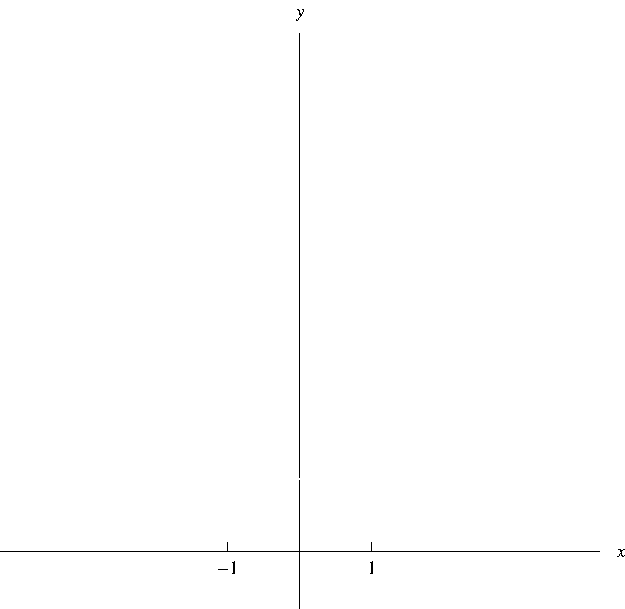
\includegraphics[height=5cm]{exponential-functions/pictures/07-02-ex7a.pdf}%
}%
\only<handout:0| 6-7>{%
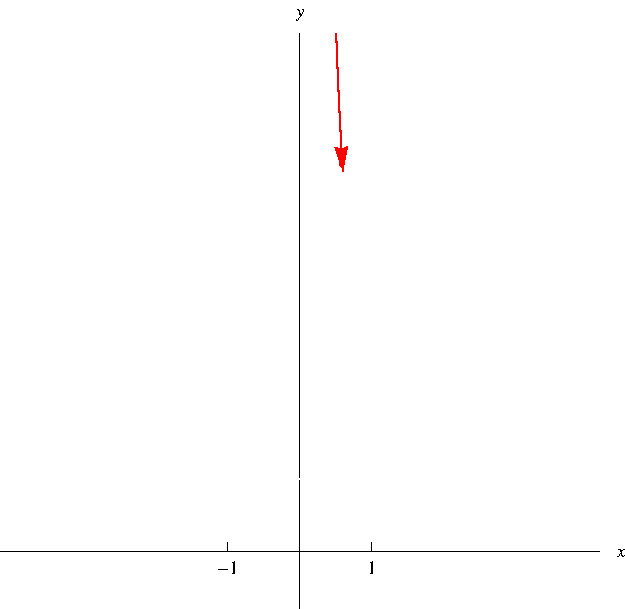
\includegraphics[height=5cm]{exponential-functions/pictures/07-02-ex7b.pdf}%
}%
\only<handout:0| 8-9>{%
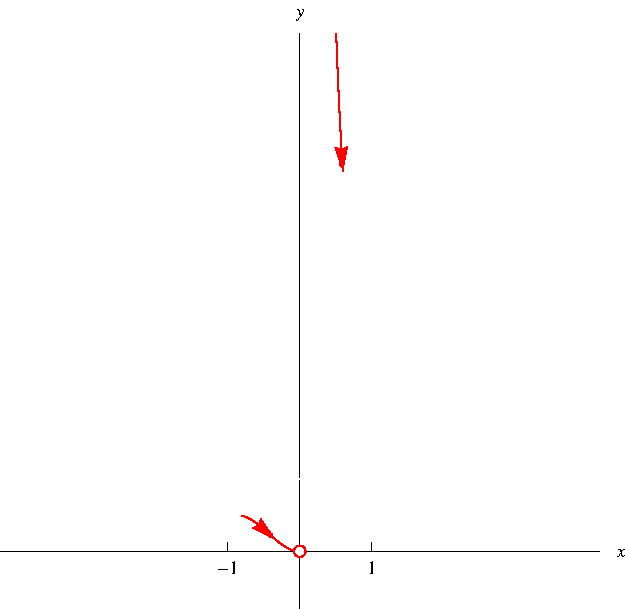
\includegraphics[height=5cm]{exponential-functions/pictures/07-02-ex7c.pdf}%
}%
\only<handout:0| 10-14>{%
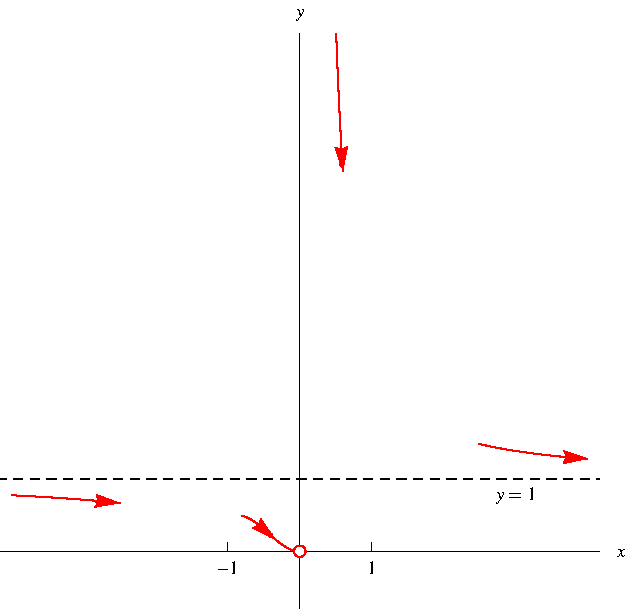
\includegraphics[height=5cm]{exponential-functions/pictures/07-02-ex7e.pdf}%
}%
\only<15->{%
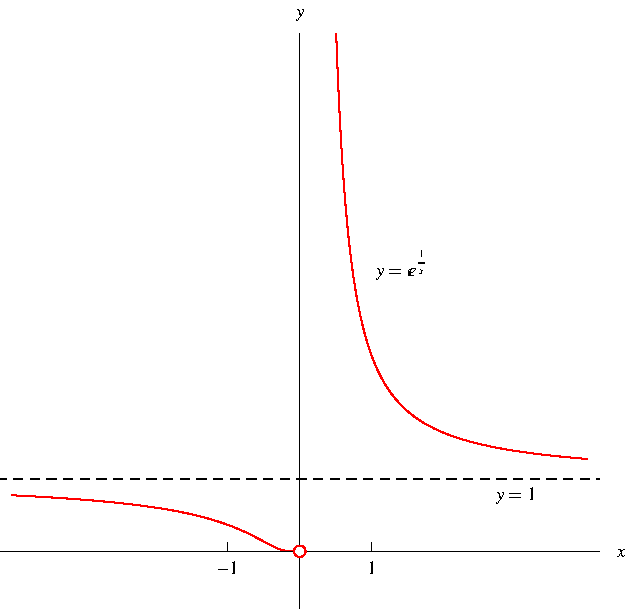
\includegraphics[height=5cm]{exponential-functions/pictures/07-02-ex7f.pdf}%
}%
\column{.6\textwidth}
\begin{itemize}
\item<2->  $f(x)$ is always positive.
\item<3->  Domain: everything but 0.
\item<4->  Check for vertical asymptote at 0.  Let $t = 1/x$.
\item<4->  $\lim_{x\rightarrow 0^+} e^{1/x} \uncover<5->{ = \lim_{t\rightarrow\infty}e^t} \uncover<6->{ = \infty .}$
\item<4->  $\lim_{x\rightarrow 0^-} e^{1/x} \uncover<7->{ = \lim_{t\rightarrow -\infty}e^t} \uncover<8->{ = 0.}$
\item<9->  As $x\rightarrow \pm \infty$, $1/x \rightarrow 0$.
\item<10->  Therefore $\lim_{x\rightarrow \pm \infty} e^{1/x} = 1$
\item<10->  $y = 1$ is a horizontal asymptote.
\end{itemize}
\end{columns}
\[
\uncover<11->{f'(x) =} \uncover<12->{-\frac{e^{1/x}}{x^2}} \uncover<13->{< 0 \textrm{ for all $x\neq 0$.}} \uncover<14->{\textrm{ Always decreasing.}}
\]
\end{example}
\end{frame}
% end module natural-exponential-ex7
